\chapter{My Work}\label{ch:MyWork}

\section{Current \ac{NAMURU} architecture}
A significant amount of time has been invested gaining an understanding of the \ac{NAMURU} receiver, its architecture and the operation of it's sub-systems. The receiver is a mixed signal device, which has been the focus of a decade of research and development. 

A detailed understanding of the receiver is crucial, if it is to be accurately modelled, in particular the ways that non idealities cause the performance of the receiver to deviate from analog models. For example, delays and jitter introduced  by the receiver's \ac{RTOS}. The Aquarius firmware developed by Glennon \cite{Glennon11aquariusfirmware} implements the tracking loop algorithm using 4,100 lines of optimised C, illustrating the complexity of the implementation.


The \ac{NAMURU} receiver uses a number of different tracking loops to track the incoming signal. During operation, the receiver transitions between a number of different states, choosing the most appropriate tracking loop at each point in time. A thorough overview of the different tracking loops employed by the receiver can be found in appendix \ref{StateTransitions}. Particular attention has been paid in this thesis to the type 3 PLL/ type 2 FLL which represents the final state for the tracking system. The type 3 PLL uses a 2nd order filter, while the type 2 FLL uses a 1st order filter. This filter architecture can be observed in figure \ref{fig:TrackingLoopeOverview}. 

\tikzset{
block/.style = {draw, fill=white, rectangle, minimum height=3em, minimum width=3em},
tmp/.style  = {coordinate}, 
sum/.style= {draw, fill=white, circle, node distance=1cm},
input/.style = {coordinate},
output/.style= {coordinate},
pinstyle/.style = {pin edge={to-,thin,black}
}
}

\begin{figure}[!htb]
\centering
\begin{tikzpicture}[auto, node distance=2cm,>=latex']
    \node [input, name=rinput] (rinput) {};
    \node [sum, right of=rinput,node distance = 2
    cm](Rotator){\Large$+$};
    \node [input, right of = Rotator] (RotatorPickoffPoint) {};
     
    
    
    %FLL Stuff
    \node [block, right of=Rotator,node distance=4cm] (DiscriminatorFLL) {$D_{FLL}$};
    \node [block, right of=DiscriminatorFLL] (SamplingTime){$\frac{1}{T}$};
    \node [block, below of = DiscriminatorFLL,node distance =6cm](K1FLL){$K_{1}$};
    \node [block, below of = K1FLL](IntegratorFLL){$\displaystyle \int$};
    \node [block, left of = IntegratorFLL](K2FLL){$K_{2}$};
    \node [sum, left of=K1FLL,node distance=2cm] (sum1FLL) {\Large$+$};
    \node [sum, left of = sum1FLL,node distance =2cm](sumCommon){\Large$+$};
    
    \node [block, above of = sumCommon](VCOIntegrator){$\displaystyle \int$};
    \node [block, above of = VCOIntegrator](VCO){VCO};
    
    
    \node [input, right of = K1FLL] (FLLPickoffPoint) {};
    
    
    
    %PLL Stuff
    \node [block, above of=DiscriminatorFLL] (DiscriminatorPLL) {$D_{PLL}$};
    \node [block, below of = IntegratorFLL](diffPLL){$\frac{d}{dt}$};
    \node [block, left of = diffPLL](K1PLL){$K_{3}$};
    \node [block, below of = diffPLL](K2PLL){$K_{4}$};
    \node [block, below of = K2PLL](IntegratorPLL){$\displaystyle \int$};
    \node [block, left of = IntegratorPLL](K3PLL){$K_{5}$};
    \node [sum, left of=K2PLL,node distance=2cm] (sum1PLL) {\Large$+$};
    \node [output, right of=DiscriminatorPLL, node distance=4cm] (output) {};
     
    
    \node [input, right of = diffPLL,node distance =4cm] (PLLPickoffPoint1) {};
    \node [input, right of = K2PLL,node distance =4cm] (PLLPickoffPoint2) {};
    
    
    %Common
    \draw [->] (rinput) -- node{$\phi_{Input}$}(Rotator);
    
    %FLL Stuff
    \draw [-] (Rotator) -- node{$\phi_{Error}$} (RotatorPickoffPoint);
    \draw [->] (RotatorPickoffPoint) -- node{} (DiscriminatorFLL);
    
    
    \draw [->] (DiscriminatorFLL) -- node{} (SamplingTime);
    
    \draw [-] (SamplingTime) |- node{} (FLLPickoffPoint);
    \draw [->] (FLLPickoffPoint) -- node{} (K1FLL);
    \draw [->] (FLLPickoffPoint) |- node{} (IntegratorFLL);
    \draw [->] (IntegratorFLL) -- node{} (K2FLL);
    
    \draw [->] (K1FLL) -- node{} (sum1FLL);
    \draw [->] (K2FLL) -- node{} (sum1FLL);
    \draw [->] (sum1FLL) -- node{} (sumCommon);
    
    
    %PLL Stuff
    \draw [->] (RotatorPickoffPoint) |- node{} (DiscriminatorPLL);
    
    \draw [-] (DiscriminatorPLL) -- node [name=y] {}(output);
    
    \draw [-] (output) -- node{} (PLLPickoffPoint1);
    \draw [-] (PLLPickoffPoint1) -- node{} (PLLPickoffPoint2);
    \draw [->] (PLLPickoffPoint1) -- node{} (diffPLL);
    \draw [->] (PLLPickoffPoint2) -- node{} (K2PLL);
    \draw [->] (PLLPickoffPoint2) |- node{} (IntegratorPLL);
   

    \draw [->] (IntegratorPLL) -- node{} (K3PLL);
    \draw [->] (diffPLL) -- node{} (K1PLL);
    
    \draw [->] (K1PLL) -- node{} (sum1PLL);
    \draw [->] (K2PLL) -- node{} (sum1PLL);
    \draw [->] (K3PLL) -- node{} (sum1PLL);
    
    \draw [->] (sum1PLL) -| node{} (sumCommon);
    \draw [->] (sumCommon) -- node{} (VCOIntegrator);
    \draw [->] (VCOIntegrator) -- node{} (VCO);
    \draw [->] (VCO) -- node{$\phi_{VCO}$} node[pos=0.90] {$-$} (Rotator);
    
    \end{tikzpicture}
\caption{An analog model of the highest level tracking loop used in the NAMURU receiver. The loop filter is parametrised by a the 5 gains, $K_1$ to $K_5$.}
\label{fig:TrackingLoopeOverview}
\end{figure}




\subsection{Some other section}





After conducting a literature review, it was decided to model the control loops used by the \ac{NAMURU} receiver in the Laplace domain. The choice of the coefficients from the tracking loop comes from a method devised by Ward \cite{Ward}. While this method is conceptually simple, requiring only a loop order and noise bandwidth as parameters, it generates robust tracking loops for most applications. Because of this, the Ward method has experienced significant popularity, amongst receiver designers.  


The method used by Ward for design will be described below for context: 

\subsection{\ac{FLL} Filter}
In the Laplace domain, we can represent the second order \ac{FLL} filter as:  $F(s) = K_1 + \frac{K_2}{s}$. The design method from Ward \cite{Ward} is used in order to determine the coefficients $K_1$ and $K_2$.  

\begin{align*}
B_n &= 6\\
a_2 &= \sqrt(2)\\
\omega_{0}&=\frac{B_n}{0.53}\\
\end{align*}

\begin{equation} \label{eq1}
\begin{split}
K_1 & = a_2 \omega_{0}\\
K_1 & = 16.00\\
\end{split}
\end{equation}

\begin{equation} \label{eq2}
\begin{split}
K_2 & = \omega_{0}^2\\
K_2 & = 128.16\\
\end{split}
\end{equation}

\subsection{\ac{PLL} Filter}
Ward's method is also used to design the co-efficients for the \ac{PLL}. In the Laplace domain, we can represent the second order filter  of the third order \ac{PLL} as : 

\begin{equation} \label{eq6}
F(s) = K_1 + \frac{K_2}{s} + \frac{K_3}{s^2}
\end{equation}

A loop bandwidth of 18Hz was originally chosen for the \ac{PLL}, as Kaplan\cite{Kaplan} demonstrated, using a Monte Carlo simulation, that higher loops bandwidths typically result in unstable behaviour. However the limiting factor for stability is the loop noise bandwidth time product. Kaplan uses an integration time of 20ms, resulting in a $BLT$ of 0.36. Conversely \ac{NAMURU} uses an integration time of 8ms, which means that any loop noise bandwidth $\leq 45$ can be used. 

Using Ward's method\cite{Ward} for finding $K_1,K_2 \& K_3$:

\begin{align*}
B_n &= 18\\
a_3&=1.1\\
b_3&=2.4\\
\omega_{0}&=\frac{B_n}{0.7845}
\end{align*}

\begin{equation} \label{eq3}
\begin{split}
K_3 & = b_3  \omega_{0}\\
    & = 55.1\\
\end{split}
\end{equation}

\begin{equation} \label{eq4}
\begin{split}
K_4 & = a_3  \omega_{0}^2\\ 
    & = 579.13\\
\end{split}
\end{equation}

\begin{equation} \label{eq5}
\begin{split}
K_5 & = \omega_{0}^3\\
    & = 12079\\
\end{split}
\end{equation}


The next stage of Laplace domain analysis after determining the transfer function of the filter is to determine the transfer function of the closed loop system.

Multiplying equation \ref{eq6} by $\frac{s^2}{s^2}$ we get :

\begin{equation}
F(s) = \frac{K_3s^2 + K_4 s + K_5}{s^2}
\end{equation}

The \ac{VCO} has the following transfer function : $G(s) = \frac{K_{vco}}{s}$


\begin{equation}
 H(s) = \frac{K_{VCO}(K_1 + \frac{K_2}{s} + \frac{K_3}{s^2})}{s+K_{VCO}(K_1 + \frac{K_2}{s} + \frac{K_3}{s^2})}
\end{equation}

Multiplying by $\frac{s^2}{s^2}$ we get :

\begin{equation}
 H(s) = \frac{K_{VCO}(K_1s^2 + K_2s + K_3)}{s^3+K_{VCO}(K_1s^2 + K_2s + K_3)}
 \end{equation}



\clearpage
\subsection{Combining FLL \& PLL}

The structure described by Ward is a combination of FLL/PLL, which operate in conjunction. This structure, which is described by Ward in his seminal paper  may initially give the impression that the FLL and PLL act independently, however a critical analysis in the Laplace domain shows that they are intricately linked\cite{Ward}.

The philosophy behind Ward's design is that the FLL will bring the frequency estimate of the tracking loop to within locking range, at which point the PLL will bring the tracking loop into phase lock. Upon further scrutiny, it becomes apparent that the PLL \& FLL form a hybrid loop, which can be analysed in the Laplace domain.


Paying particular attention to figure \ref{fig:TrackingLoopeOverview}, we can observe the PLL and FLL arms of the loop controller. The blocks $D_{PLL}$ and $D_{FLL}$ represent the PLL and FLL discriminators respectively. More information about the implementation of these discriminators can be found in appendix \ref{app:Discriminators}. 


\tikzset{
block/.style = {draw, fill=white, rectangle, minimum height=3em, minimum width=3em},
tmp/.style  = {coordinate}, 
sum/.style= {draw, fill=white, circle, node distance=1cm},
input/.style = {coordinate},
output/.style= {coordinate},
pinstyle/.style = {pin edge={to-,thin,black}
}
}

\begin{figure}[!htb]
\centering
\begin{tikzpicture}[auto, node distance=2cm,>=latex']
    \node [input, name=rinput] (rinput) {};
    \node [sum, right of=rinput,node distance = 2
    cm](Rotator){\Large$+$};
    \node [input, right of = Rotator] (RotatorPickoffPoint) {};
     
    
    
    %FLL Stuff
    \node [block, right of=Rotator,node distance=4cm] (DiscriminatorFLL){$S$};
    \node [input, right of=DiscriminatorFLL] (SamplingTime){};
    \node [block, below of = DiscriminatorFLL,node distance =8cm](K1FLL){$K_{1}$};
    \node [block, below of = K1FLL](IntegratorFLL){$\frac{1}{S}$};
    \node [block, left of = IntegratorFLL](K2FLL){$K_{2}$};
    \node [sum, left of=K1FLL,node distance=2cm] (sum1FLL) {\Large$+$};
    \node [sum, left of = sum1FLL,node distance =2cm](sumCommon){\Large$+$};
    
    \node [block, above of = sumCommon](VCOIntegrator){$\frac{1}{S}$};
    \node [block, above of = VCOIntegrator](VCOGain){$K_{VCO}$};
    \node [block, above of = VCOGain](VCO){$\frac{1}{S}$};
    
    
    \node [input, right of = K1FLL] (FLLPickoffPoint) {};
    
    
    
    %PLL Stuff
    \node [block, above of=DiscriminatorFLL] (DiscriminatorPLL) {$1$};
    \node [block, below of = IntegratorFLL](diffPLL){$S$};
    \node [block, left of = diffPLL](K1PLL){$K_{3}$};
    \node [block, below of = diffPLL](K2PLL){$K_{4}$};
    \node [block, below of = K2PLL](IntegratorPLL){$\frac{1}{S}$};
    \node [block, left of = IntegratorPLL](K3PLL){$K_{5}$};
    \node [sum, left of=K2PLL,node distance=2cm] (sum1PLL) {\Large$+$};
    \node [output, right of=DiscriminatorPLL, node distance=4cm] (output) {};
     
    
    \node [input, right of = diffPLL,node distance =4cm] (PLLPickoffPoint1) {};
    \node [input, right of = K2PLL,node distance =4cm] (PLLPickoffPoint2) {};
    
    
    %Common
    \draw [->] (rinput) -- node{$\phi_{Input}$}(Rotator);
    
    %FLL Stuff
    \draw [-] (Rotator) -- node{$\phi_{Error}$} (RotatorPickoffPoint);
    \draw [->] (RotatorPickoffPoint) -- node{} (DiscriminatorFLL);
    
    
    \draw [-] (DiscriminatorFLL) -- node{} (SamplingTime);
    
    \draw [-] (SamplingTime) |- node{} (FLLPickoffPoint);
    \draw [->] (FLLPickoffPoint) -- node{} (K1FLL);
    \draw [->] (FLLPickoffPoint) |- node{} (IntegratorFLL);
    \draw [->] (IntegratorFLL) -- node{} (K2FLL);
    
    \draw [->] (K1FLL) -- node{} (sum1FLL);
    \draw [->] (K2FLL) -- node{} (sum1FLL);
    \draw [->] (sum1FLL) -- node{} (sumCommon);
    
    
    %PLL Stuff
    \draw [->] (RotatorPickoffPoint) |- node{} (DiscriminatorPLL);
    
    \draw [-] (DiscriminatorPLL) -- node [name=y] {}(output);
    
    \draw [-] (output) -- node{} (PLLPickoffPoint1);
    \draw [-] (PLLPickoffPoint1) -- node{} (PLLPickoffPoint2);
    \draw [->] (PLLPickoffPoint1) -- node{} (diffPLL);
    \draw [->] (PLLPickoffPoint2) -- node{} (K2PLL);
    \draw [->] (PLLPickoffPoint2) |- node{} (IntegratorPLL);
   

    \draw [->] (IntegratorPLL) -- node{} (K3PLL);
    \draw [->] (diffPLL) -- node{} (K1PLL);
    
    \draw [->] (K1PLL) -- node{} (sum1PLL);
    \draw [->] (K2PLL) -- node{} (sum1PLL);
    \draw [->] (K3PLL) -- node{} (sum1PLL);
    
    \draw [->] (sum1PLL) -| node{} (sumCommon);
    \draw [->] (sumCommon) -- node{} (VCOIntegrator);
    \draw [->] (VCOIntegrator) -- node{} (VCOGain);
    \draw [->] (VCOGain) -- node{} (VCO);
    \draw [->] (VCO) -- node{$\phi_{VCO}$} node[pos=0.90] {$-$} (Rotator);
    
    

    \end{tikzpicture}
\caption{A Laplace domain model of figure \ref{fig:TrackingLoopeOverview}. Note that the FLL discriminator is equivalent to a differentiation, or S in the Laplace domain, conversely, the VCO is replaced by an integrator.} 
\label{fig:TrackingLoopeOverviewLaplace}
\end{figure}


\tikzset{
block/.style = {draw, fill=white, rectangle, minimum height=3em, minimum width=3em},
tmp/.style  = {coordinate}, 
sum/.style= {draw, fill=white, circle, node distance=1cm},
input/.style = {coordinate},
output/.style= {coordinate},
pinstyle/.style = {pin edge={to-,thin,black}
}
}

\begin{figure}[!htb]
\centering
\begin{tikzpicture}[auto, node distance=2cm,>=latex']
    \node [input, name=rinput] (rinput) {};
    \node [sum, right of=rinput,node distance = 2
    cm](Rotator){\Large$+$};
    \node [input, right of = Rotator] (RotatorPickoffPoint) {};
     
    
    
    %FLL Stuff
   
    \node [block, right of=Rotator,node distance =4cm] (SamplingTime){$\frac{1}{T}$};
    
    \node [block, below of = SamplingTime,node distance =8cm](K1FLL){$K_{1}$};
    
    \node [block, below of = K1FLL](IntegratorFLL){$\frac{1}{S}$};
    \node [block, left of = IntegratorFLL](K2FLL){$K_{2}$};
    \node [sum, left of=K1FLL,node distance=2cm] (sum1FLL) {\Large$+$};
    \node [sum, left of = sum1FLL,node distance =2cm](sumCommon){\Large$+$};
    
    \node [block, above of = VCOIntegrator](VCOGain){$K_{VCO}$};
    \node [block, above of = VCOGain](VCO){$\frac{1}{S}$};
    
    
    \node [input, right of = K1FLL] (FLLPickoffPoint) {};
    
    
    
    %PLL Stuff
    \node [block, above of=SamplingTime] (DiscriminatorPLL) {$1$};
    
    \node [block, left of = diffPLL](K1PLL){$K_{3}$};
    \node [block, below of = diffPLL](K2PLL){$K_{4}$};
    \node [block, right of = K2PLL](ExtraIntegrator){$\frac{1}{S}$};
    
    \node [block, below of = K2PLL](IntegratorPLL){$\frac{1}{S^2}$};
    \node [block, left of = IntegratorPLL](K3PLL){$K_{5}$};
    \node [sum, left of=K2PLL,node distance=2cm] (sum1PLL) {\Large$+$};
    \node [output, right of=DiscriminatorPLL, node distance=4cm] (output) {};
     
    
    \node [input, right of = diffPLL,node distance =4cm] (PLLPickoffPoint1) {};
    \node [input, right of = K2PLL,node distance =4cm] (PLLPickoffPoint2) {};
    
    
    %Common
    \draw [->] (rinput) -- node{$\phi_{Input}$}(Rotator);
    
    %FLL Stuff
    \draw [-] (Rotator) -- node{$\phi_{Error}$} (RotatorPickoffPoint);
    \draw [->] (RotatorPickoffPoint) -- node{} (SamplingTime);
    
    
    \draw [-] (SamplingTime) -| node{} (FLLPickoffPoint);
    \draw [->] (FLLPickoffPoint) -- node{} (K1FLL);
    \draw [->] (FLLPickoffPoint) |- node{} (IntegratorFLL);
    \draw [->] (IntegratorFLL) -- node{} (K2FLL);
    
    \draw [->] (K1FLL) -- node{} (sum1FLL);
    \draw [->] (K2FLL) -- node{} (sum1FLL);
    \draw [->] (sum1FLL) -- node{} (sumCommon);
    
    
    %PLL Stuff
    \draw [->] (RotatorPickoffPoint) |- node{} (DiscriminatorPLL);
    
    \draw [-] (DiscriminatorPLL) -- node [name=y] {}(output);
    
    \draw [-] (output) -- node{} (PLLPickoffPoint1);
    \draw [-] (PLLPickoffPoint1) -- node{} (PLLPickoffPoint2);
    \draw [->] (PLLPickoffPoint1) -- node{} (K1PLL);
    \draw [->] (PLLPickoffPoint2) -- node{} (ExtraIntegrator);
    \draw [->] (ExtraIntegrator) -- node{} (K2PLL);
    
    \draw [->] (PLLPickoffPoint2) |- node{} (IntegratorPLL);
   

    \draw [->] (IntegratorPLL) -- node{} (K3PLL);
    %\draw [->] (diffPLL) -- node{} (K1PLL);
    
    \draw [->] (K1PLL) -- node{} (sum1PLL);
    \draw [->] (K2PLL) -- node{} (sum1PLL);
    \draw [->] (K3PLL) -- node{} (sum1PLL);
    
    
    \draw [->] (sum1PLL) -| node{} (sumCommon);
    \draw [->] (sumCommon) -- node{} (VCOGain);
    %\draw [->] (VCOIntegrator) -- node{} (VCOGain);
    \draw [->] (VCOGain) -- node{} (VCO);
    \draw [->] (VCO) -- node{$\phi_{VCO}$} node[pos=0.90] {$-$} (Rotator);
    
    

    \end{tikzpicture}
\caption{A Laplace domain model of figure \ref{fig:TrackingLoopeOverview}. Note that the FLL discriminator is equivalent to a differentiation, or S in the Laplace domain, conversely, the VCO is replaced by an integrator.} 
\label{fig:ModifiedStructure}
\end{figure}


\tikzset{
block/.style = {draw, fill=white, rectangle, minimum height=3em, minimum width=3em},
tmp/.style  = {coordinate}, 
sum/.style= {draw, fill=white, circle, node distance=1cm},
input/.style = {coordinate},
output/.style= {coordinate},
pinstyle/.style = {pin edge={to-,thin,black}
}
}

\begin{figure}[!htb]
\centering
\begin{tikzpicture}[auto, node distance=2cm,>=latex']
    \node [input, name=rinput] (rinput) {};
    \node [sum, right of=rinput,node distance = 2cm](Rotator){\Large$+$};
    \node [block, below of =Rotator](VCO){$\frac{1}{S}$};
    
    %PLL Stuff
  
    
    \node at (4,-6) [sum] (sum1PLL) {\Large$+$};
  
    \node [block, above of = sum1PLL](K1PLL){$\frac{K_{1}}{T} + K_{3}$};
    \node [block, right of = sum1PLL](K2PLL){$\frac{K_{2}}{T} + K_{4}$};
    \node [block, right of = K2PLL](ExtraIntegrator){$\frac{1}{S}$};
    
    \node [block, below of = K2PLL](IntegratorPLL){$\frac{1}{S^2}$};
    \node [block, left of = IntegratorPLL](K3PLL){$K_{5}$};
    
     
    
    \node [input, right of = K1PLL,node distance =6cm] (PLLPickoffPoint1) {};
    \node [input, right of = K2PLL,node distance =4cm] (PLLPickoffPoint2) {};
    
    
    %Common
    \draw [->] (rinput) -- node{$\phi_{Input}$}(Rotator);
    \draw [-] (Rotator) -| node{} (PLLPickoffPoint1);
    
    
    \draw [-] (PLLPickoffPoint1) -- node{} (PLLPickoffPoint2);
    \draw [->] (PLLPickoffPoint1) -- node{} (K1PLL);
    \draw [->] (PLLPickoffPoint2) -- node{} (ExtraIntegrator);
    \draw [->] (ExtraIntegrator) -- node{} (K2PLL);
    
    \draw [->] (PLLPickoffPoint2) |- node{} (IntegratorPLL);

    \draw [->] (IntegratorPLL) -- node{} (K3PLL);
   
    
    \draw [->] (K1PLL) -- node{} (sum1PLL);
    \draw [->] (K2PLL) -- node{} (sum1PLL);
    \draw [->] (K3PLL) -- node{} (sum1PLL);

    \draw [->] (sum1PLL) -| node{} (VCO);
    \draw [->] (VCO) -- node{$\phi_{VCO}$} node[pos=0.90] {$-$} (Rotator);
    
    \end{tikzpicture}
\caption{The reduced block diagram, to simplify the diagram, we assume that $K_{VCO}=1$.} 
\label{fig:ModifiedStructure2}
\end{figure}


From figure \ref{fig:ModifiedStructure2} we can find the open loop transfer function as:

\begin{equation}
\frac{1}{s} (\frac{K_1}{T}+K_3 + \frac{1}{s}(\frac{K_2}{T}+K_4) + \frac{1}{s^2} K_5)
\label{eq:CombinedOpenLoopTF}
\end{equation}

We can convert the open loop transfer function $F(s)$ to the closed loop transfer function $H(s)$ as follows\cite{KazemiPHD}\cite{Gardner}:

\begin{equation}
 H(s) = \frac{K_{VCO}F(s)}{1+K_{VCO}F(s)}
\end{equation}

Assuming $K_{VCO}=1$:

\begin{equation}
 H(s) = \frac{F(s)}{1+F(s)}
\label{eq:OpenLoopToClosedLoop}
\end{equation}

Substituting equation \ref{eq:CombinedOpenLoopTF} into equation \ref{eq:OpenLoopToClosedLoop}:

\begin{equation}
 H(s) = \frac{\frac{1}{s} (\frac{K_1}{T}+K_3 + \frac{1}{s}(\frac{K_2}{T}+K_4) + \frac{1}{s^2} K_5)}{1+\frac{1}{s} (\frac{K_1}{T}+K_3 + \frac{1}{s}(\frac{K_2}{T}+K_4) + \frac{1}{s^2} K_5)}
\end{equation}

\begin{equation}
 H(s) = \frac{s^2(\frac{K_1}{T}+K_3) + s(\frac{K_2}{T}+K_4) + K_5}
 {s^3+ s^2(\frac{K_1}{T}+K_3)+ s(\frac{K_2}{T}+K_4) + K_5}
\end{equation}
\clearpage


From Wards method \cite{Ward}, we have the following coefficients:

\begin{align*}
K_1 &=\frac{\sqrt{2}B_{nFLL}}{0.53}\\
    &= 2.668 B_{nFLL}
\end{align*}

\begin{align*}
K_2 &=\frac{B_{nFLL}^2}{0.53^2}\\
    &= 0.2809 B_{nFLL}^2
\end{align*}

\begin{align*}
K_3 &=\frac{2.4B_{nPLL}}{0.7845}\\ 
    &=3.059 B_{nPLL}\\
\end{align*}

\begin{align*}
K_4 &=\frac{1.1B_{nPLL}^2}{0.7845^2}\\
    &=1.787 B_{nPLL}^2
\end{align*}

\begin{align*}
K_5 &=\frac{B_{nPLL}^3}{0.7845^3}\\
    &=0.4828B_{nPLL}^3
\end{align*}

It is clear at this point 


\subsection{Euler integration Approximation}

\begin{equation}
s \approx \Big(\frac{z-1}{Tz}\Big)
\end{equation}



\begin{equation}
 H(s) = \frac{s^2(K1) + s(K2) + K3}
 {s^3+ s^2(K1)+ s(K2) + K3}
\end{equation}


\begin{equation}
 H(s) = \frac{\Big(\frac{z-1}{Tz}\Big)^2(K1) + \Big(\frac{z-1}{Tz}\Big)(K2) + K3}{\Big(\frac{z-1}{Tz}\Big)^3+ \Big(\frac{z-1}{Tz}\Big)^2(K1)+ \Big(\frac{z-1}{Tz}\Big)(K2) + K3}
\end{equation}

My Equation
\begin{equation}
\frac{\frac{K_{1}}{t} + K_{3} + \frac{K_{5}}{s^{2}} + \frac{1}{s} \left(\frac{K_{2}}{t} + K_{4}\right)}{s \left(1 + \frac{1}{s} \left(\frac{K_{1}}{t} + K_{3} + \frac{K_{5}}{s^{2}} + \frac{1}{s} \left(\frac{K_{2}}{t} + K_{4}\right)\right)\right)}
\end{equation}

\begin{equation}
\frac{K_{1} s^{2} + K_{3} s^{2} t + K_{5} t + s \left(K_{2} + K_{4} t\right)}{K_{1} s^{2} + K_{3} s^{2} t + K_{5} t + s^{3} t + s \left(K_{2} + K_{4} t\right)}
\end{equation}

\begin{equation}
\frac{T z \left(K_{1} \left(z - 1\right)^{2} + K_{3} t \left(z - 1\right)^{2} + K_{5} T^{2} t z^{2} + T z \left(K_{2} + K_{4} t\right) \left(z - 1\right)\right)}{T z \left(K_{1} \left(z - 1\right)^{2} + K_{3} t \left(z - 1\right)^{2} + K_{5} T^{2} t z^{2} + T z \left(K_{2} + K_{4} t\right) \left(z - 1\right)\right) + t \left(z - 1\right)^{3}}
\end{equation}

\clearpage

Book Example

\begin{equation}
\frac{1.0 z \left(14.48 z^{2} - 28.21 z + 13.73\right)}{15.48 z^{3} - 31.21 z^{2} + 16.73 z - 1.0}
\end{equation}



\clearpage




















\section{Ward Analysis}

From Kazemi, \cite{Kazemi2008}, the Loop Noise Bandwidth time product ($B_L T$) must be less than 0.55. 
For an 8ms integration time, we have 

\begin{align*}
B_n &\leq \frac{0.55}{0.008} \text{ (Hz)}\\
    &\leq 68.75 \text{ (Hz)}
\end{align*}

\subsection{PLL}
Kaplan suggests that "A conservative rule of thumb for tracking threshold is that the 3-sigma jitter must not exceed one-fourth of the phase pull-in range of the PLL discriminator." %\cite{Kaplan}

\begin{equation}
3 \sigma_{PLL} = 3 \sigma_j +\theta_e \leq 45 \degree
\end{equation}

Where:
\begin{align*}
\sigma_j &= \text{1-sigma phase jitter from all sources except dynamic stress error} \\
\theta_e &= \text{dynamic stress error in the PLL tracking loop}
\end{align*}

%\cite{Kaplan}
\begin{equation}
\sigma_{PLL} = \sqrt{\sigma^2_{tPLL} + \sigma^2_v+ \theta^2_A} + \frac{\theta_e}{3} \leq 15 \degree 
\end{equation}
%\cite{Jwo}

Where:
\begin{align*}
\sigma_{tPLL} &= \text{1-sigma thermal noise (degrees)}\\
\sigma_v &= \text{1-sigma vibration-induced oscillator jitter (degrees)}\\
\theta_A &= \text{Allan variance induced oscillator jitter (degrees)}
\end{align*}
%\cite{Kaplan}\cite{Jwo}


\begin{equation}
\sigma_{PLLt} = \frac{360}{2 \pi} \sqrt{\frac{B_n}{C/N_0}(1+\frac{1}{2 \cdot T \cdot C/N_0})} \text{ (degrees)}
\end{equation}
%\cite{Kaplan}

Where:
\begin{align*}
B_n &= \text{carrier loop noise bandwidth (Hz)} \\
C/N_0 &= \text{carrier to noise power ratio in (Hz)} \\
&=10^\frac{(C/N_0)_dB}{10} \text{ Hz}\\
T &= \text{pre-detection (coherent) integration time (s)} \\
\lambda_L &= \text{GPS L1 carrier wavelength (m)}\\
&= 0.1903 \text{ m}
\end{align*}


\begin{equation}
\theta_e = \frac{360 \cdot d^3R/dt^3  \cdot f_L}{c  \cdot \omega^3_0} \text{ (degrees)}
\end{equation}


Where:
\begin{align*}
\omega &= \frac{B_n}{0.7845} \\
f_L &= \text{L-band input frequency in Hz (1575.42MHz)}\\ 
c & = 2.99792458 \times 10^8 ms^{-1}
\end{align*}




\begin{equation}
\theta_{A3} = 160 \frac{\sigma_A(\tau)f_L}{B_n} \text{ (degrees)}
\end{equation}

Where:
\begin{align*}
\sigma_A(\tau) &= 10 \times 10^{-10} \text{ (dimensionless units of }\Delta f/f\text{)}
\end{align*}

From \cite{VT803Datasheet}


\begin{equation}
\theta_{A3} =\frac{25.2}{B_n} \text{ (degrees)}
\end{equation}

For $B_n$ =18, we have $\theta_{A3}=1.4\degree$.


\begin{figure}[!htb] 
    \centering
    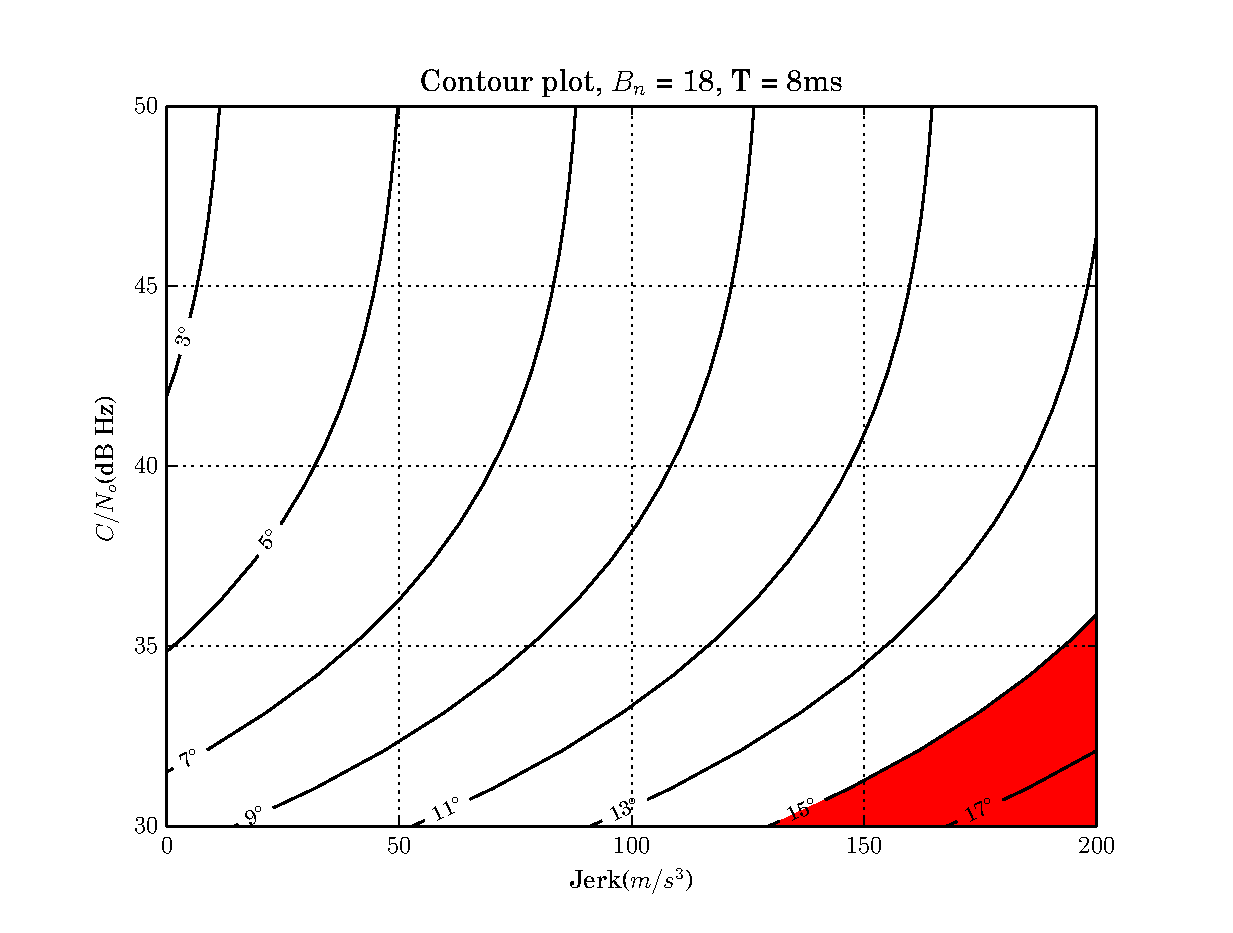
\includegraphics[width=1\textwidth]{mywork/18ContourPLL.eps} 
    \caption{A contour plot for a 3rd order loop with a $B_n$ of 18Hz. A value of $1.4\degree$ for the Allan variance oscillator jitter and $1.8\degree$ for vibration oscillator jitter is used. The conservative threshold of 15\degree can be seen in red. From this, we can conclude that the loop is likely to loose phase lock at a $C/N_0$ of 30,  at a jerk of $150ms^{-3}$.}
\end{figure}

\begin{figure}[!htb] 
    \centering
    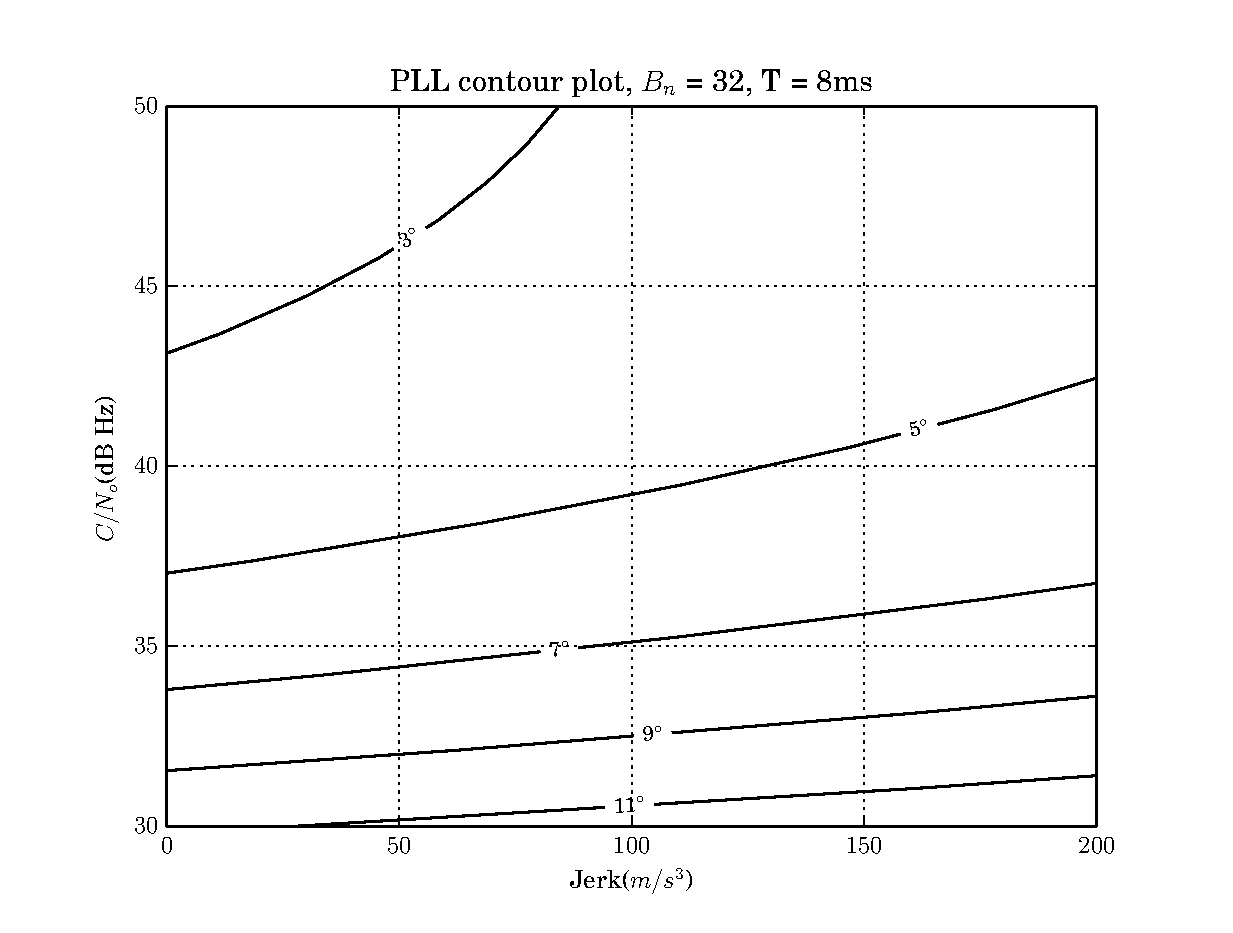
\includegraphics[width=1\textwidth]{mywork/32ContourPLL.eps} 
    \caption{A value of $1.4\degree$ for the Allan variance oscillator jitter and $1.8\degree$ for vibration oscillator jitter is used.}
\end{figure}


\begin{figure}[!htb] 
    \centering
    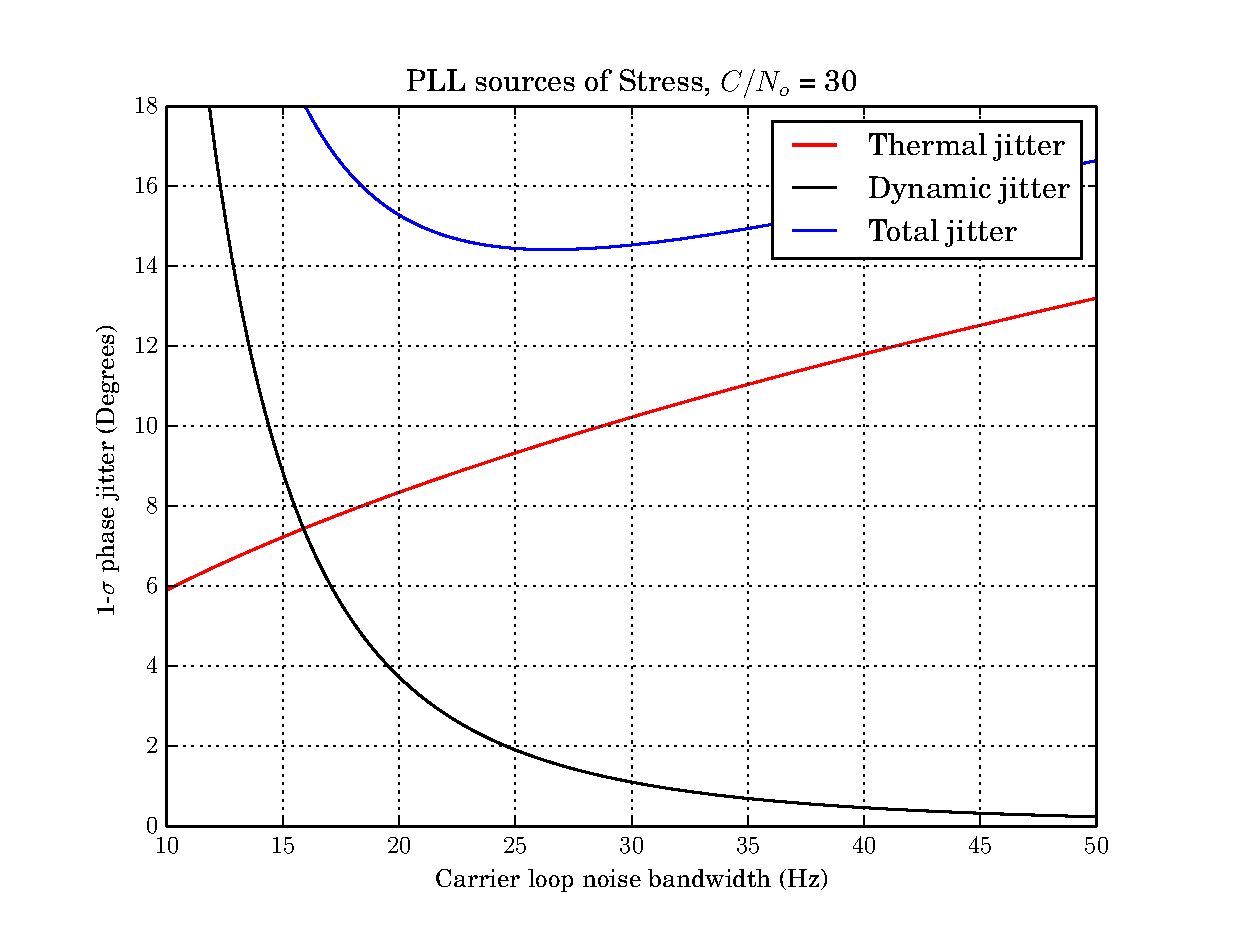
\includegraphics[width=1\textwidth]{mywork/PLLStresses.eps} 
    \caption{This plot breaks down the sources of error. Note that the phase jitter is at a minimum for a value of $B_n$ equal to approximately 27.}
\end{figure}


\subsection{FLL}


Talk about this
5.6.2 FLL Tracking Loop Measurement Errors

Generate figure 5.24
Generate figure 5.25

Also talk about section 5.6.2

\begin{equation}
\sigma_{FLL} =  \sigma_{tFLL} + \frac{f_e}{3} \leq \frac{T}{12} \text{ (Hz)}
\end{equation}

For T = 4ms, we have $\sigma_{FLL} \leq 20.83$ Hz.


Where:
\begin{align*}
\sigma_{tFLL} &= \text{1-sigma thermal noise frequency jitter}\\
f_e &= \text{dynamic stress error in the FLL tracking loop}
\end{align*}


\begin{equation}
\sigma_{tFLL} = \frac{1}{2 \pi T} \sqrt{ \frac{4FB_n}{C/N_0}(1 + \frac{1}{TC/N_0})} \text{ (Hz)}
\end{equation}

\begin{align*}
F &= \text{1 at high } C/N_0\\
  &= \text{2 near threshold}
\end{align*}


\begin{equation}
f_e = \frac{d}{dt}(\frac{1}{360 \omega^n_0}\frac{d^nR}{dt^n}) = \frac{1}{360\omega^n_0} \frac{d^{n+1}R}{dt^{n+1}} \text{ (Hz)}
\end{equation}


\begin{figure}[!htb] 
    \centering
    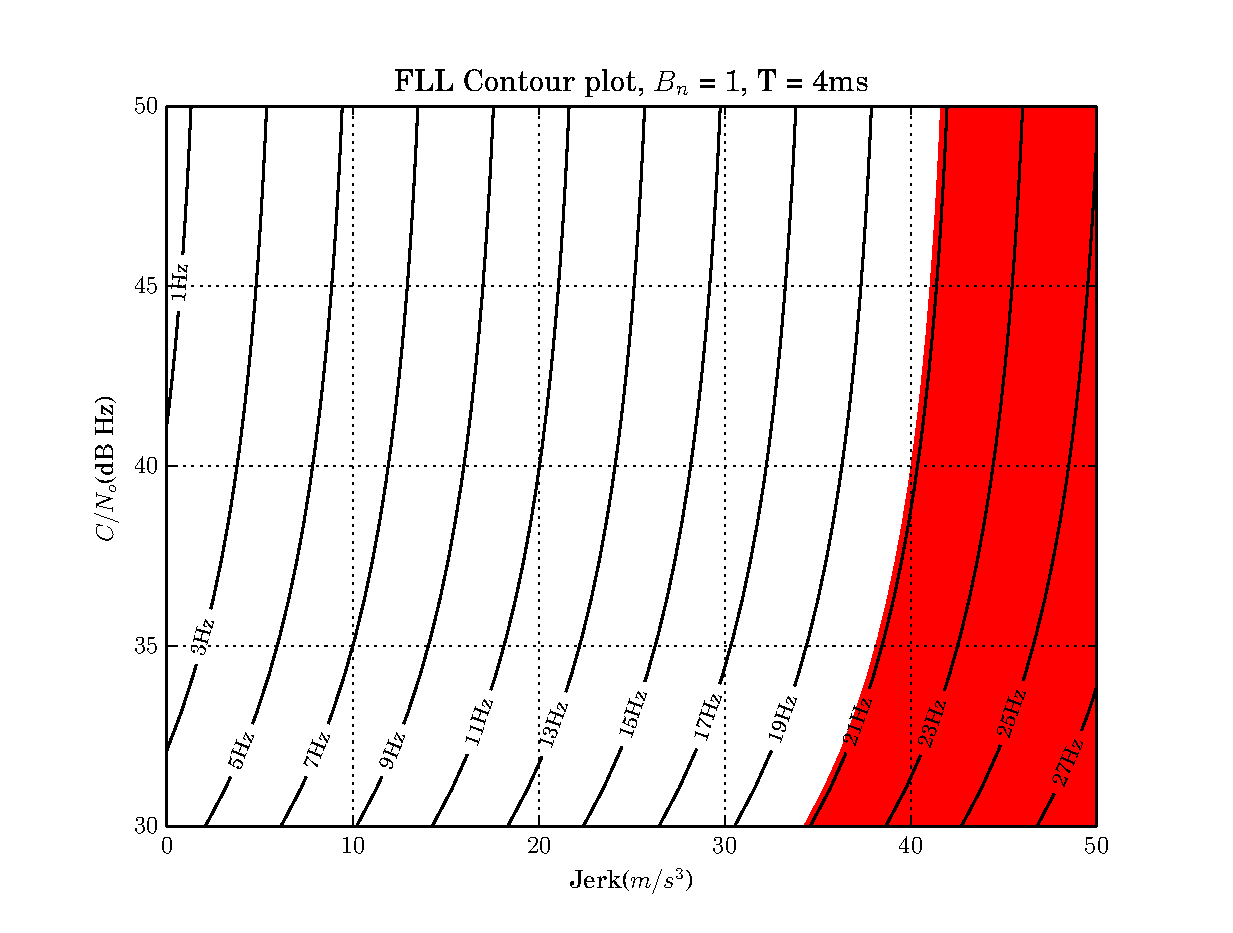
\includegraphics[width=1\textwidth]{mywork/1ContourFLL.eps} 
    \caption{The cutoff for the FLL is 20.83 Hz.}
\end{figure}

\begin{figure}[!htb] 
    \centering
    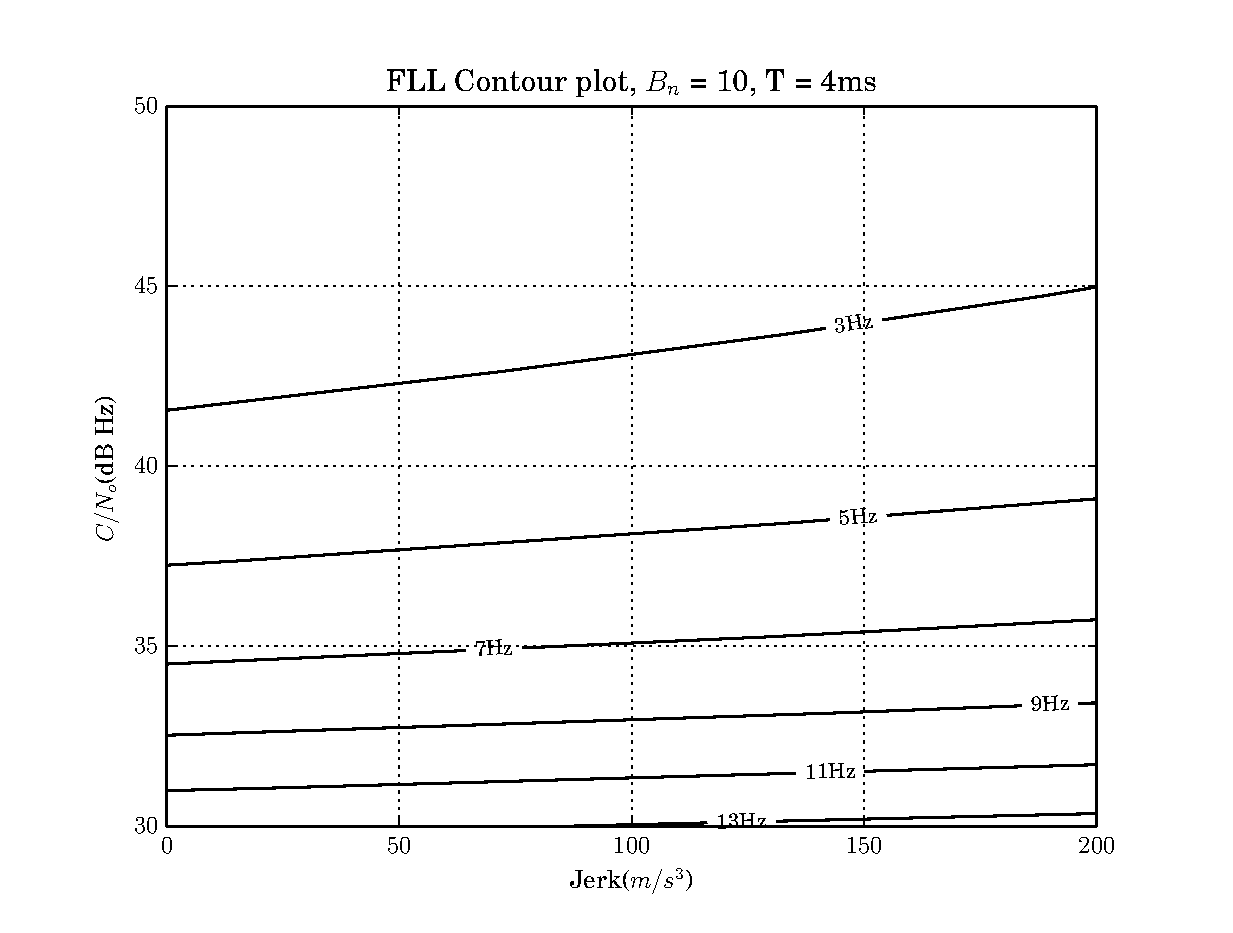
\includegraphics[width=1\textwidth]{mywork/10ContourFLL.eps} 
    \caption{}
\end{figure}



\begin{figure}[!htb] 
    \centering
    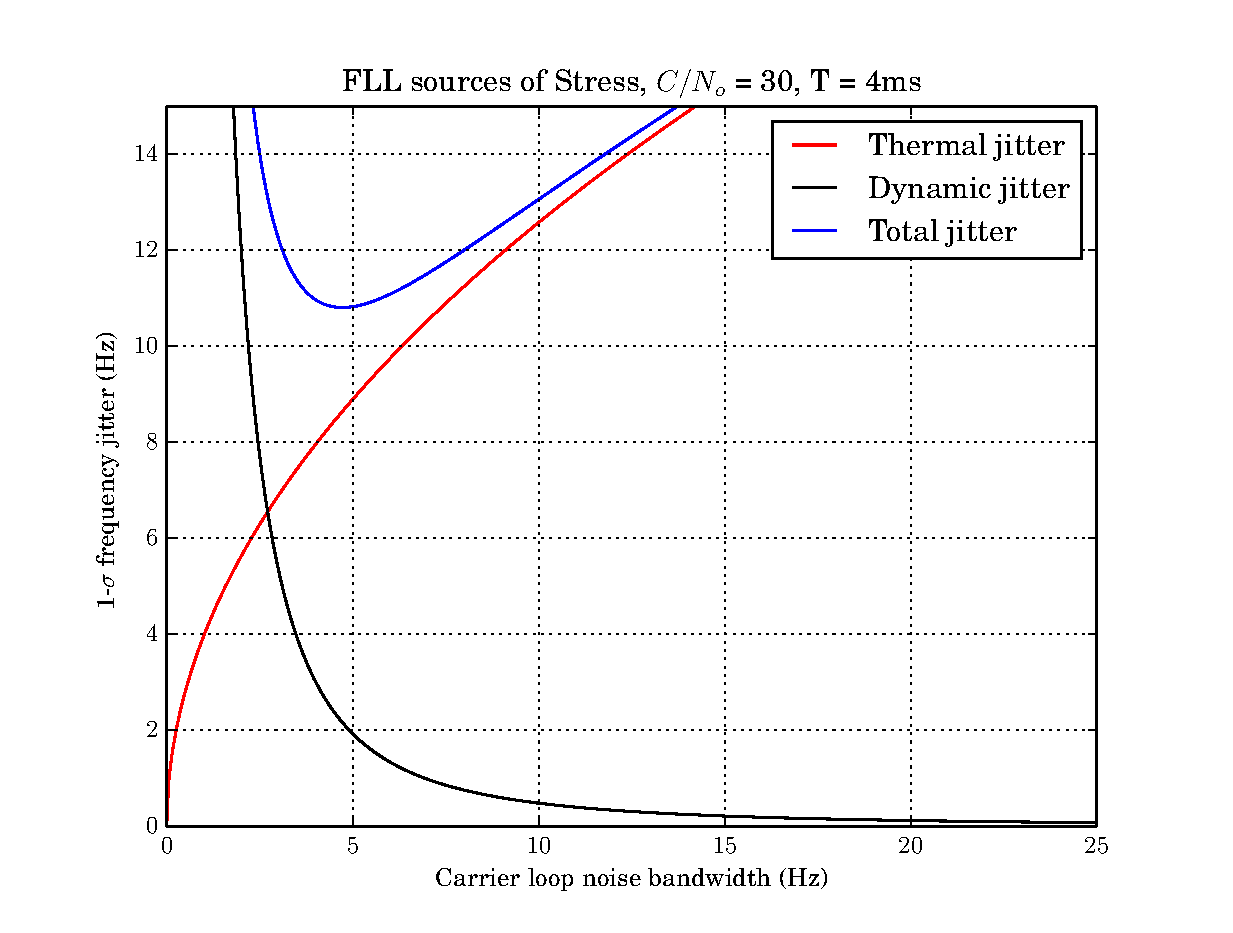
\includegraphics[width=1\textwidth]{mywork/FLLStresses.eps} 
    \caption{This plot breaks down the sources of error. Note that the phase jitter is at a minimum for a value of $B_n$ equal to approximately 27.}
\end{figure}




Significant preliminary work has been carried out, because of the challenging scope of thesis. 

In order to have a rigorous understanding of the dynamic performance of the \ac{NAMURU} receiver, we must first examine the theoretical basis for the operation of its tracking loops. 

A model of the operation of the tracking loops can be established by building upon intellectual foundations laid in continuous time control theory. While this Laplace domain model provides an idealised understanding of the \ac{PLL}, it does not take into the effects of delay and jitter in the loop. 

\ac{PLL}, \ac{FLL} and \ac{DLL} are all examples of control systems. By convention, what is referred to in the parlance of control theory as a "controller" is referred to as the "loop filter" in \ac{GNSS} related literature. One key point to keep in mind with a \ac{PLL} is that a phase input results in a frequency output. This effective integration occurs in the \ac{VCO}.

\section{Zeros and Poles}
The behaviour of a closed loop system is determined by the locations of the zeros and the poles. In particular, their location determines if the system is stable for all possible inputs. Even if the system is found not to be stable for all possible inputs, it may be stable for all \emph{reasonable} inputs. An important caveat is that the location of the zeros and poles is for an analog model of the system, the locations will be different for a digital model, with the difference in location depending on the $B_LT$ product.  Hence it is possible to design a system which is stable in the Laplace domain but unstable in the Z Domain. 

Root locus provides an efficient graphical method for analysing the stability of a system in the Laplace domain\cite{Nise}. Matlab was used to generate a Root Locus plot of the current Laplace domain model of the \ac{PLL} implementation using the following code:

\begin{comment}
\begin{lstlisting}[frame=single]
Kvco =1;
Bn = 18;
a3 = 1.1;
b3 = 2.4;
omega = Bn/0.7845;
k1 = b3*omega;
k2 = a3*(omega^2);
k3 = omega^3;
%H is the forward transfer function
H = tf([Kvco*k1 Kvco*k2 Kvco*k3],[1 0 0 0]);
rlocus(H);
\end{lstlisting}
\end{comment}

\begin{comment}
The results of this analysis can be seen in figure \ref{fig:RootLocus}, from this analysis of the root locus, we can determine  that the system is stable, for values of the \ac{VCO} gain which are larger than 0.38. This is an important result, as intuitively, increasing the gain will typically make a system unstable. However, this result demonstrates the value of Root Locus analysis for evaluating the stability of a higher order system.

In order to verify the implementation of the analog model was correct, a second graphical model was constructed in CircuitLab. This model can be seen in figure \ref{fig:gpsLoopModel}. By adjusting the VCO gain, the threshold between stable and unstable behaviour for a step input was confirmed to be 0.38. The results from this experiment can be seen in figures \ref{fig:Stable} and \ref{fig:Unstable}

Additionally, this model confirmed that the current\ac{NAMURU} architecture is able to integrate up velocity and acceleration however it is vulnerable to Jerk. This was assessed by applying ramp and parabolic inputs to the input, and comparing to the output.
\end{comment}

\section{Simulation}

\subsection{Hardware simulation}
A software based receiver has been developed as part of the thesis, in order to gain a greater understanding of the performance of tracking loops on real world data. 

The software receiver was developed in python, based on the authors previous experience with the language, as well the need to interface with domain specific libraries. 
The approach of using an \ac{GNSS}, and testing in software was effectively used by Kazemi \cite{KazemiPHD} in order to critically evaluate the performance of the new tracking loops developed as part of his PHD.

A signal was generated by a Spirent \ac{GPS} simulator, which can be seen in figure \ref{fig:Spirent}. This signal was then digitised using a NordNav \ac{SDR}, with a sampling rate of $16.3676 \times 10^6$ samples per second. 

A range of simulations were created in order to better understand the performance of the software receiver. In particular, scenarios for 0g, 1g, 2g, 5g, 7.5g and 10g were created. In figure \ref{fig:Doppler}, the output from the \ac{NCO} of the software receiver can be seen. In the simulation, the receiver remains stationary until 8s, at which point it starts acceleration directly upwards at 10g, creating a ramp in the \ac{NCO} frequency. It is important to note that while the receiver is accelerating at 10g, the \ac{LOS} dynamics may only be 5g. 

\begin{figure}[!htb] 
    \centering
    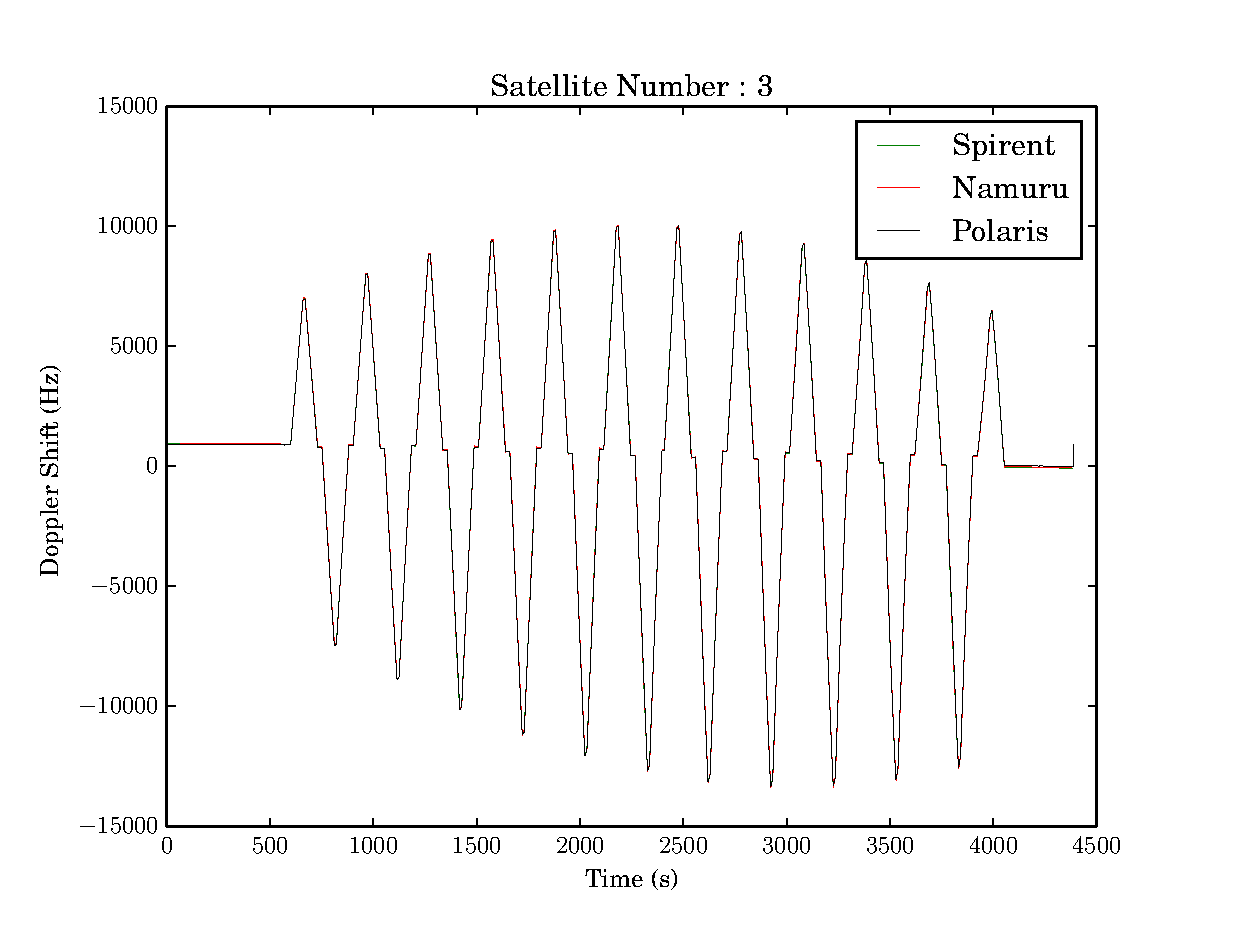
\includegraphics[width=1\textwidth]{PolarisCharts/3Polaris.eps} 
    \caption{An example of a simulation. The receiver undergoes a sequence of increasing accelerations, which }
    \label{fig:Polaris3}
\end{figure}


\begin{figure}[!htb] 
    \centering
    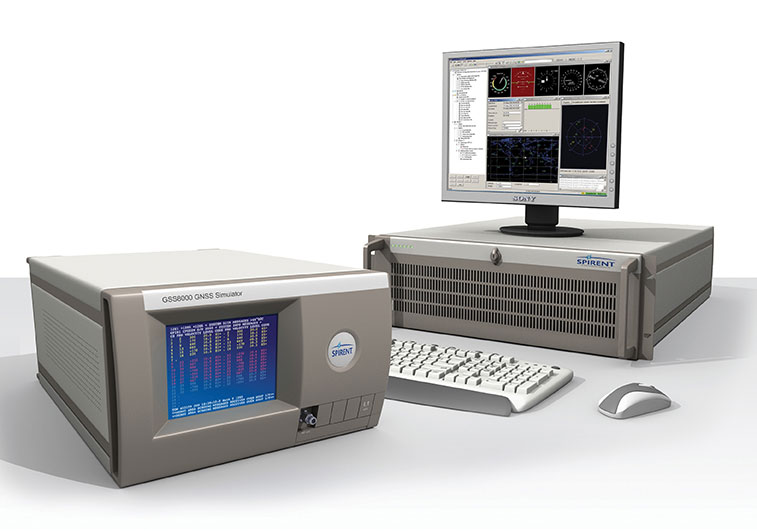
\includegraphics[width=1\textwidth]{mywork/Spirent-GSS8000.jpg} 
    \caption{An example of a Spirent \ac{GPS} simulator. The actual model used differs from the one pictured.}
    \label{fig:Spirent}
\end{figure}

\begin{figure}[!htb] 
    \centering
    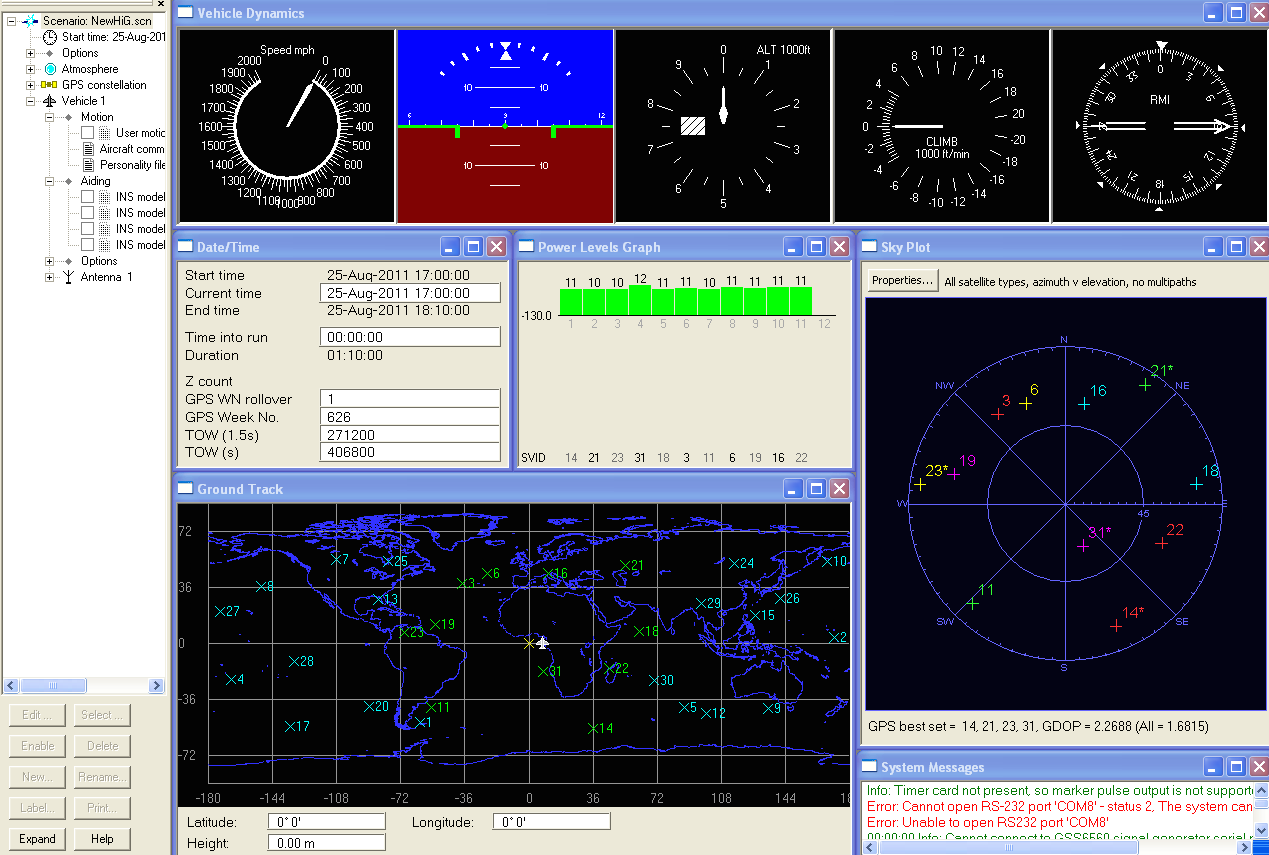
\includegraphics[width=1\textwidth]{mywork/HighGScreenshot.png} 
    \caption{The SimGen software, used to define scenarios and control the \ac{GNSS} simulator.}
    \label{fig:HighGScreenshot}
\end{figure}


The correct performance of a \ac{PLL} can be examined by attempting to decode the navigation message transmitted by the satellite. Other, more sophisticated methods for determining if the  receiver is in phase lock, will be examined in Thesis B. In figures \ref{fig:RawSignal} and \ref{fig:DigitalSignal}, the decoded message can be clearly seen, indicating that the receiver is maintaining phase lock with the signal.

\subsection{Software simulation}
\ref{app:Code}

\section{Airborne Experiment}

\begin{figure}[!htb] 
    \centering
    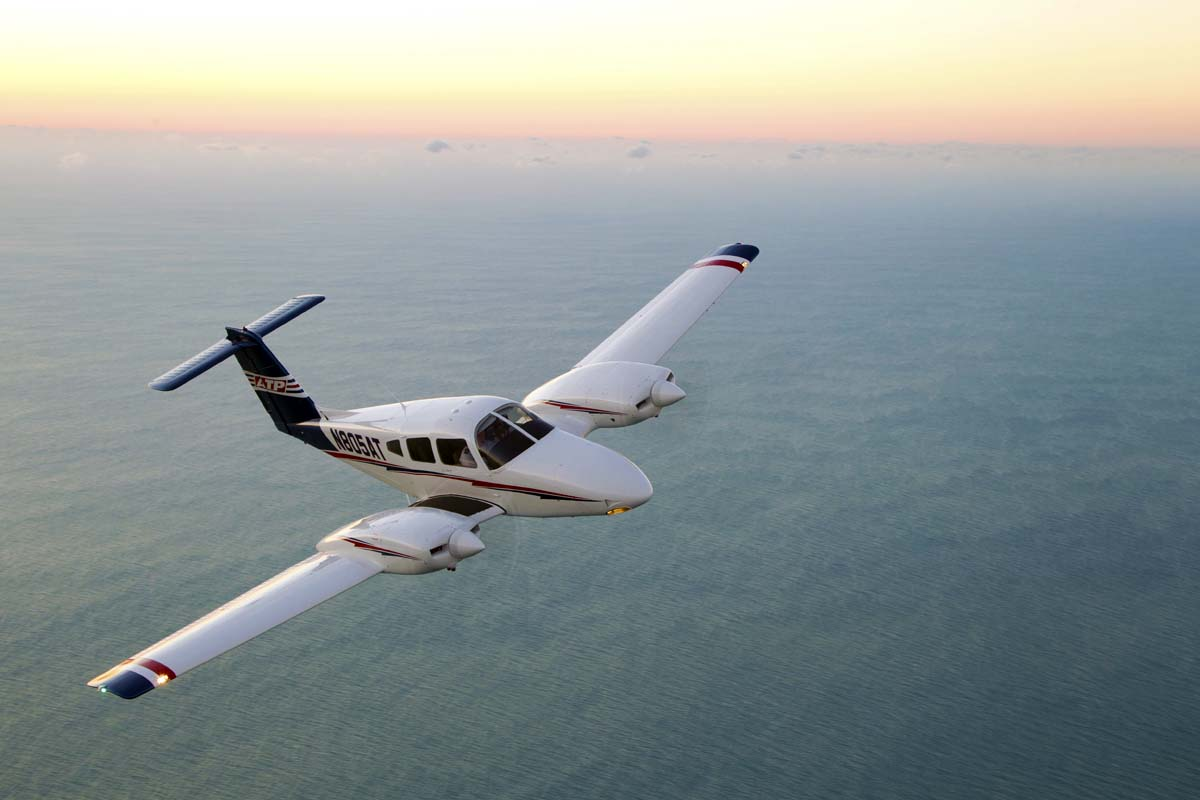
\includegraphics[width=1\textwidth]{mywork/SeminoleBankingPRjpg.jpg} 
    \caption{A Piper PA-44 Seminole.}
    \label{fig:PiperSeminole}
\end{figure}

A real-world data-set was processed, consisting of data taken captured a flight aboard a UNSW Aviation Piper PA-44 Seminole VH-FRI. Data from the flight was captured by a NordNav IF Recorder, and processed using the the software receiver. 

The actual carrier doppler shift, as measured by taking the finite difference of the satellite pseudoranges, and converted to Hz, was compared against the measured Doppler shift in the software receiver. There is a small offset because of drift in the receiver crystal. The results of this experiment can be see in figure \ref{fig:SimulatedDynamics}. While the dynamics experienced by the receiver were on the order of $\pm 5m/s^2$, somewhat less than the dynamics that are experienced by a \ac{LV}, This experiment is important, as it verifies the real world performance of the soft receiver. 



\section{My Stuff}

CNO = 45

PLLBW =32
FLLBW = 10
76.135, std = 2.3549

PLLBW = 18
FLLBW = 1
128.26,std =  2.59 

PLLBW = 32
FLLBW = 0
131.6 std = 1.64


